\documentclass{CLGPY}


\usepackage{listings}
\usepackage{cncolours}
\lstset{
    basicstyle=\small\ttfamily,%整体格式设置
    columns=fullflexible,%设置字符列为非等宽
    breaklines=true,%自动换行
    % frameround=ttff,%边框四角弧度,t则弧
    frame=tb,%边框样式
    backgroundcolor=\color{赤金!15},%背景颜色
    framerule=1.5pt,%边框线宽度
    rulecolor=\color{墨色},%边框线颜色
    % framesep=.5em,%边距
    numbers=left,%左边显示数字
    % numbersep=0em,
    xleftmargin=2em,
    framexleftmargin=2em,
    numberstyle={\sffamily\footnotesize\color{teal}}
}

\lstdefinelanguage{latex}{
    morecomment=[l]{\%},
    commentstyle=\color{lightgray},
    morekeywords={begin,end},
    keywordstyle=\color{blue!50!black},
    morekeywords={[2]documentclass,usepackage},%导言区命令
    keywordstyle={[2]\color{red!75!black}},
    morekeywords={[3]juanqi,title,author,institute,sxrq,jjxm,zzjj,txzz,xinxi,Title,Author,Institute,keywords,enkeywords,document,abstract,enabstract,minipage,tabular,tikzpicture,multicols,includegraphics,caption,captionof,center,quad,qquad,parbox,centering,subcaption,animateinline,bibliographystyle,cite,nocite,bibliography,textbf,enumerate,itemize,toprule,bottomrule,midrule,thebibliography,bibitem,small,footnotesize,verb},%命令和环境
    keywordstyle={[3]\color{cyan!70!black}},
    morekeywords={[4]maketitle,Maketitle,figure,table},
    keywordstyle={[4]\color{朱红}},
    morekeywords={[5]CLGPY,ctexart,ctexbook,ctexrep,book,article,report,standalone,tikz,tikz-3dplot,animate,ctex,fontspec,multicol,caption,subcaption,natbib,float,booktabs,geometry,graphicx,color,xcolor,hyperref,amsmath,mathtools,siunitx,mathabx},%文类和宏包
    keywordstyle={[5]\color{竹青}},
    morekeywords={[6]part,chapter,section,subsection,subsubsection,paragraph,subparagraph},%章节
    keywordstyle={[6]\color{琥珀}},
    morekeywords={[7],newcommand,newenvironment,renewcommand,renewenvironment,def,edef,gdef,xdef}%定义类命令
    keywordstyle={[7]\color{blue!70!black}},
}
\lstnewenvironment{latexcode}
{\lstset{language=latex}}
{}%代码设置,定义了用来排版LaTeX代码的latexcode环境
%%---------------------字体设置--------------------%

% 注意:如果希望使用\ctexset 在导言区指定字库,则需要先在宏包/文档类选项中指定fontset = none(这会禁用CTEX 宏集的操作系统检测功能和自动设定字库功能)
\setCJKmainfont[ItalicFont={FZKai-Z03},BoldFont={FZHei-B01},BoldItalicFont=FZLiShu-S01S]{FZShuSong-Z01}%设置正文字体为宋体,其粗体为黑体、斜体为楷体、粗斜为隶书,全文的一种设置
\setCJKsansfont{FZHei-B01}%设置无衬线字体为黑体
% \setCJKmonofont{}%设置打字机字体
%设置字体族
\setCJKfamilyfont{zhsong}{FZShuSong-Z01}
\setCJKfamilyfont{zhhei}{FZHei-B01}
\setCJKfamilyfont{zhkai}{FZKai-Z03}
\setCJKfamilyfont{zhfs}{FZFangSong-Z02}
%带*的\newcommand*不能有\par
\def\songti{\CJKfamily{zhsong}} % 宋体
\def\heiti{\CJKfamily{zhhei}} % 黑体
\def\kaishu{\CJKfamily{zhkai}} % 楷书
\def\fangsong{\CJKfamily{zhfs}} % 仿宋
%--------------------------------------------------%%字体设置
%--------------------以下命令是为了写说明文档而定义的,实际使用时可不管------------------------------%
\def\ts#1{\textcolor{red}{#1}}%提示命令
\def\bzx#1#2{$\underbracket[.5pt][1pt]{\text{#1}}_{\textcolor{red}{\text{#2}}}$}%下标注命令
\def\bzs#1#2{$\overbrace{\text{#1}}^{\textcolor{red}{\text{#2}}}$}%上标注命令
% \def\xbz#1#2{\vtop{\halign{##\crcr \hfil #1\hfil\crcr \noalign{\nointerlineskip\textcolor{red}{\hrule}\kern1pt} \hfil\small\textcolor{red}{#2}\hfil\crcr}}}%一个失败的尝试
\def\BibTeX{{%
\rm
B%
\kern-.05em%
{%
\sc
i%
\kern-.025em %
b%
}%
\kern-.08em
T%
\kern-.1667em%
\lower.7ex\hbox{E}%
\kern-.125em%
X%
}}%bibtex样式定制%为了写说明文档而定义的几个命令

%--------------------------使用说明----------------------%
%注:\juanqi、\title、\author三条命令必须要有,不然系统会终止编译
%\juanqi{X}{X}%卷期填写,命令\juanqi{<卷>}{<期>}
\title[布料仿真]{布料仿真:加速的十年}%标题填写,命令\title[<想要出现在奇数页页眉的标题,若缺省则默认为正式标题>]{<正式标题>}
\author[]{\textsuperscript{1}}%作者填写,命令\author[<想要出现在奇数页页眉的作者,若缺省则默认为正式作者>]{<正式作者>}
\institute{({})}%机构填写,命令\institute{<机构>}
\begin{document}
    \maketitle%生成题名页并修改题名页页眉
    \begin{abstract}%中文摘要环境
        本文主要介绍布料仿真的常见方法以及近十年布料仿真的前沿研究,包括对已有算法的性能优化、新的仿真算法,以及算法在GPU上的并行化实现,总结了当前布料仿真的前沿方向
    \end{abstract}
    \keywords{布料仿真}%中文关键词命令
    %\xinxi{O 4–1\ts{(参照:\url{http://www.ztflh.com}})}{\bzx{A}{作者抄写}}{\bzx{1000-0712}{作者抄写} \bzx{XXXXXX}{编辑填写}}{\bzx{10.16854/j.cnki.1000-0712.}{作者抄写} \bzx{XXXXXX}{编辑填写}}%一些必要信息填写,命令\xinxi{<中图分类号>}{<文献标识码>}{<文章编号>}{<【DOI】>}
    \begin{multicols}{2}%以下部分内容采用双栏排版
        \section{布料仿真的常见方法}
        \subsection{弹簧质点系统}
        布料在发生形变时,需要考虑系统内部的相对影响,通过弹簧可以模拟布料形变时产生的弹性势能。首先将布料用网格表示,给网格的顶点一定的质量,通过弹簧将网格的顶点相连构成弹簧质点系统。
        \begin{center}
            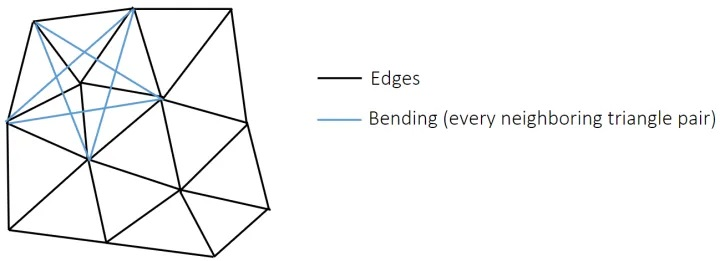
\includegraphics[width=1.0\linewidth]{./fig/弹簧质点模型.jpg}
            \captionof{figure}{弹簧质点模型}
        \end{center}

        在不考虑非保守力的作用下,系统中质点的位置可以唯一地确定系统的状态。利用牛顿第二定律:
        \begin{equation}
			x''=M^{-1}(\frac{\partial E}{\partial x})
        \end{equation}

        在存在非保守力时:
        \begin{equation}
            x''=M^{-1}(\frac{\partial E}{\partial x}+F)
        \end{equation}

		在弹簧质点系统中,根据胡克定律(Hooke's law):
        \begin{equation}
		\begin{split}
			&F_{spring}=-k_s\Delta x \\
			&F_{s_i}=k_s(1-\frac{L}{\left \| x_i-x_j \right \| })(x_i-x_j)
		\end{split}
        \end{equation}
​		除此之外还可以加入重力、空气阻力、弹簧阻尼等其它作用力。

​		在模拟系统随时间的演化时,求解(2)式得到:
        \begin{equation}
            x = \iint M^{-1}(\frac{\partial E}{\partial x}+F)dtdt=\iint adtdt
        \end{equation}

		在实际的模拟中,时间是离散的,因此需要做数值积分。直接的方法是显式欧拉方法(explicit Euler method):
        \begin{equation}
		\begin{split}
			v(i+1) = v(i) + a(i)\Delta t \\
			x(i+1) = x(i) + v(i)\Delta t
		\end{split}
        \end{equation}
		此时下一时刻的速度和位移完全由上一时刻决定,导致当$\Delta t$较大时计算结果不稳定。

		另一种方法是隐式欧拉方法(implicit Euler method):
        \begin{equation}
		\begin{split}
			v(i+1) = v(i) + a(i+1)\Delta t \\
			x(i+1) = x(i) + v(i+1)\Delta t
		\end{split}
        \end{equation}
		由于加速度也是位置的函数,此时需要解方程得出下一时刻的速度,它的误差比显式欧拉方法小一些。

		在隐式欧拉方法中,将速度方程代入位置方程可以得到:
		\begin{equation}
		\begin{split}
			x(i+1) &= x(i) + (v(i) + a(i+1)\Delta t)\Delta t\\
       		&= x(i) + v(i)\Delta t + a(i+1)(\Delta t)^2\\
       		&= x(i) + v(i)\Delta t + M^{-1}f(i+1)(\Delta t)^2
		\end{split}
		\end{equation}
        \begin{equation}
			\frac{M}{(\Delta t)^2}(x(i+1)-x(i)-v(i)\Delta t) - f(i+1)=0
        \end{equation}

		在不考虑非保守力时,可以构造一个优化问题,使$x(i+1)$为这个优化问题的解,从而利用求解优化问题的方法求解数值积分:
		\begin{equation}
		\begin{split}
			&F(x)=\frac{1}{2(\Delta t)^2}(x-\bar x)^TM(x-\bar x)+E(x)\\
			&\bar x=x(i)+v(i)\Delta t\\
			&x(i+1) = \mathop{argmin}\limits_xF(x)
		\end{split}
		\end{equation}
		求解式(8)等价于求解$F(x)$的导数为0的点,从而转化为求解$F(x)$的极值。

		考虑系统可能发生的碰撞,最终需要求解的问题为:
		\begin{equation}
		\begin{split}
			&x(i+1) = \mathop{argmin}\limits_xF(x)\\
			&s.t. \quad x(i+1) \in  \Omega
		\end{split}
		\end{equation}

		当系统与连续体发生碰撞时:
        \begin{equation}
			s.t. \quad tx(i+1) +(1-t)x(i) \in  \Omega \quad t\in[0,1]
        \end{equation}

		为了求解这个优化问题,可以使用牛顿法,利用下面的公式进行迭代直到收敛:
        \begin{equation}
			x^{k+1} = x^{k}-(\nabla ^2F(x))^{-1}\nabla F(x)
        \end{equation}
		初始的$x^0=x(i)$,最终收敛的$x^{k}=x(i+1)$

		\subsection{弹性模型}
		将布料抽象成三角形的网格,处理当三角形网络发生形变时所带来的的能量变化:

		\begin{itemize}
			\item[$\bullet$] 当三角形的边长改变时需要能量
			\item[$\bullet$] 当两个相邻三角形的夹角发生变化时需要能量
			\item[$\bullet$] 当三角形需要变形或剪切时需要能量
		\end{itemize}

		在能量发生变化时需要相应的力做功,因此可以通过系统的状态推出系统内部各质点之间的相互作用力。

		可以通过建模的方式来计算相应的力,将相互作用力视作边长、相邻三角形二面角的函数。
        \begin{center}
            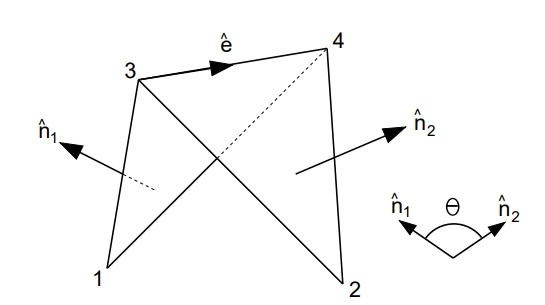
\includegraphics[width=1.0\linewidth]{./fig/二面角.jpg}
            \captionof{figure}{二面角}
        \end{center}

		首先u1和u2应该在法线方向n1和n2,其次弯曲不会拉伸边缘x3x4,因此u4-u3应该与边缘正交,即为n1和n2的线性组合。根据牛顿定律,合,力应为0,综上所述得到计算结果:
		\begin{equation}
		\begin{array}{l}
		\mathbf{u}_{1}=\|\mathbf{E}\| \frac{\mathbf{N}_{1}}{\left\|\mathbf{N}_{1}\right\|^{2}} \\
		\mathbf{u}_{2}=\|\mathbf{E}\| \frac{\mathbf{N}_{2}}{\left\|\mathbf{N}_{2}\right\|^{2}} \\
		\mathbf{u}_{3}=\frac{\left(\mathbf{x}_{1}-\mathbf{x}_{4}\right) \cdot \mathbf{E}}{\|\mathbf{E}\|} \frac{\mathbf{N}_{1}}{\left\|\mathbf{N}_{1}\right\|^{2}}+\frac{\left(\mathbf{x}_{2}-\mathbf{x}_{4}\right) \cdot \mathbf{E}}{\|\mathbf{E}\|} \frac{\mathbf{N}_{2}}{\left\|\mathbf{N}_{2}\right\|^{2}} \\
		\mathbf{u}_{4}=-\frac{\left(\mathbf{x}_{1}-\mathbf{x}_{3}\right) \cdot \mathbf{E}}{\|\mathbf{E}\|} \frac{\mathbf{N}_{1}}{\left\|\mathbf{N}_{1}\right\|^{2}}-\frac{\left(\mathbf{x}_{2}-\mathbf{x}_{3}\right) \cdot \mathbf{E}}{\|\mathbf{E}\|} \frac{\mathbf{N}_{2}}{\left\|\mathbf{N}_{2}\right\|^{2}}
		\end{array}
		\end{equation}

		得到以下有关力的函数
        \begin{equation}
			{\mathbf{f}}_{i}=k\frac{\|\mathbf{E}\Vert^{2}}{\|\mathbf{N}_{1}\|+\|\mathbf{N}_{2}\|}\mathrm{sin}\left(\frac{\pi-\theta}{2}\right)\mathbf{u}_{i}
        \end{equation}

		也可以在相邻三角形上加上弹簧以抵抗弯曲。

        \begin{center}
            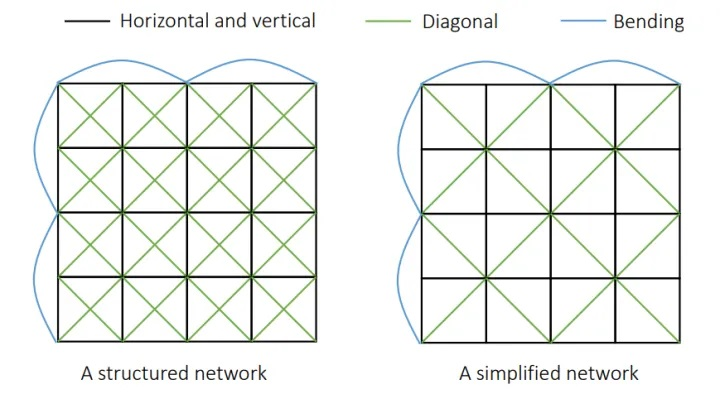
\includegraphics[width=1.0\linewidth]{./fig/三种弹簧.jpg}
            \captionof{figure}{三种弹簧}
        \end{center}

		质点弹簧模型和其他弯曲模型,假设布料平面变形(伸缩)和布料弯曲变形是独立的,相互不影响,但是实际上并非如此。 Locking issue: 如下图,当弹簧stiffnes很大(即很难形变的时候),右边的网格很难弯曲。
        \begin{center}
            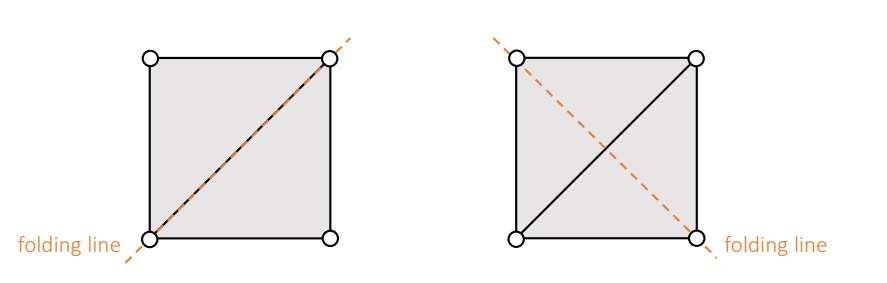
\includegraphics[width=1.0\linewidth]{./fig/Locking issue.jpg}
            \captionof{figure}{Locking issue}
        \end{center}

		为了解决这个问题,弹簧在压缩的时候,可以将弹性系数设置的小一点。或者让弹簧在一定范围内没有力,可以自由伸缩。

		\subsection{基于位置的动力学方法}

		基于位置的动力学方法(PBD)的算法流程如下
        \begin{center}
            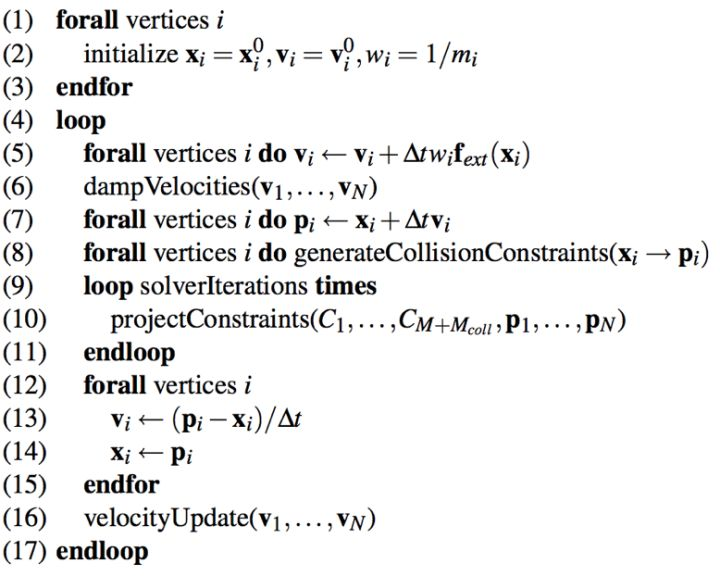
\includegraphics[width=1.0\linewidth]{./fig/PBD算法.jpg}
            \captionof{figure}{PBD算法}
        \end{center}

		每次迭代时,首先根据外力算出此时的速度更新,然后让速度根据阻尼衰减,再根据速度得到位移的变化量,通过位移生成碰撞约束,之后在位移的基础上对约束条件进行迭代直到收敛,再根据位移变化得出最终的速度。

		其中算法的核心是在位移的基础上对约束条件进行迭代直到收敛,这里将之前得到的预估位移投影到约束条件上从而得到最终位移。

		假设有一个n维约束:
		\begin{equation}
		\begin{split}
			&\pmb{p} = [\pmb{p_1},…,\pmb{p_n}]\\
			&C(\pmb{p}) = 0
		\end{split}
		\end{equation}

		现在需要找到偏移量$\Delta \pmb{p}$,使得投影前的$\pmb{p}$在偏移后满足约束:
        \begin{equation}
			C(\pmb{p}+\Delta \pmb{p})=0
        \end{equation}

		对约束函数在$\pmb{p}$处进行展开:
        \begin{equation}
			C(\pmb{p}+\Delta \pmb{p}) = C(\pmb{p}) + \nabla_pC(\pmb{p}) \cdot \Delta \pmb{p} +o(\Delta \pmb{p}) =0
        \end{equation}

		将$\Delta \pmb{p}$限定在$\nabla_pC(\pmb{p})$的方向上可以保持动量、角动量守恒:
        \begin{equation}
			\Delta \pmb{p} = \lambda \nabla_pC(\pmb{p})
        \end{equation}

		联立可得:
        \begin{equation}
			\Delta \pmb{p} = -\frac{C(\pmb{p})}{\left | \nabla_pC(\pmb{p}) \right | ^2}\nabla_pC(\pmb{p})
        \end{equation}

		对于单个质点来说:
        \begin{equation}
		\Delta \pmb{p_i} = -\frac{C(\pmb{p})}{\sum_{j} \left | \nabla_{p_j}C(\pmb{p}) \right | ^2}\nabla_{p_i}C(\pmb{p})
        \end{equation}

		考虑到质点的$\Delta \pmb{p_i}$应与质量的倒数$\omega_i=\frac{1}{m_i}$成反比
        \begin{equation}
\Delta \pmb{p_i} = -\frac{C(\pmb{p})}{\sum_{j} \omega_j\left | \nabla_{p_j}C(\pmb{p}) \right | ^2}\omega_i\nabla_{p_i}C(\pmb{p})
        \end{equation}

		对于布料,两个质点之间的距离约束可以表述为:
        \begin{equation}
			C(\pmb{p_1},\pmb{p_2})=\left | \pmb{p_1}-\pmb{p_2} \right |-L
        \end{equation}

		梯度为:
		\begin{equation}
		\begin{split}
			&\nabla_{p_1}C(\pmb{p_1},\pmb{p_2})=\frac{\pmb{p_1}-\pmb{p_2}}{\left | \pmb{p_1}-\pmb{p_2} \right |}\\
			&\frac{C(\pmb{p})}{\sum_{j} \omega_j\left | \nabla_{p_j}C(\pmb{p}) \right | ^2} = \frac{\left | \pmb{p_1}-\pmb{p_2} \right |-L}{2}
		\end{split}
		\end{equation}

		约束投影后的偏移为:
        \begin{equation}
		\Delta \pmb{p_1} =-\frac{1}{2}(\left | \pmb{p_1}-\pmb{p_2} \right |-L)\frac{\pmb{p_1}-\pmb{p_2}}{\left | \pmb{p_1}-\pmb{p_2} \right |}
        \end{equation}

		以下为两种迭代的方法,其中Gauss-Seidel遍历全部约束,难以进行并行。
        \begin{center}
            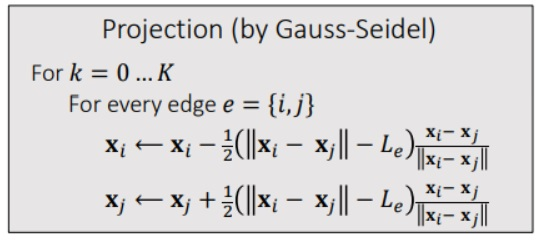
\includegraphics[width=1.0\linewidth]{./fig/PBD(Gauss-Seidel).jpg}
            \captionof{figure}{PBD(Gauss-Seidel)}
        \end{center}

		Jacobi方法在遍历全部约束后统一更新。
        \begin{center}
            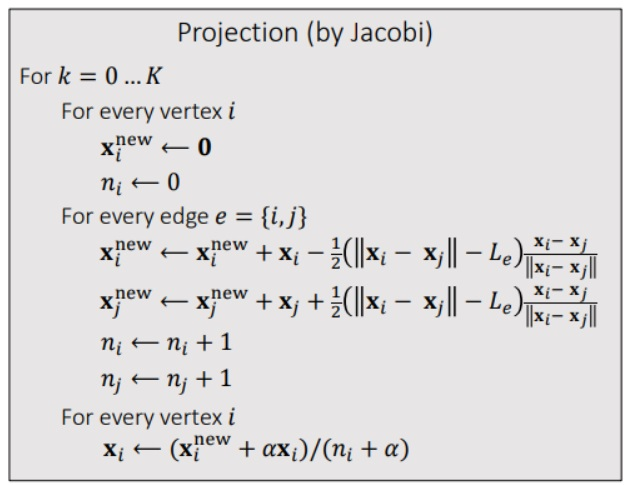
\includegraphics[width=1.0\linewidth]{./fig/PBD(Jacobi).jpg}
            \captionof{figure}{PBD(Jacobi)}
        \end{center}
		
		对于两个约束Ci和Cj,Gauss-Seidel和Jacobi方法的直观对比如下
        \begin{center}
            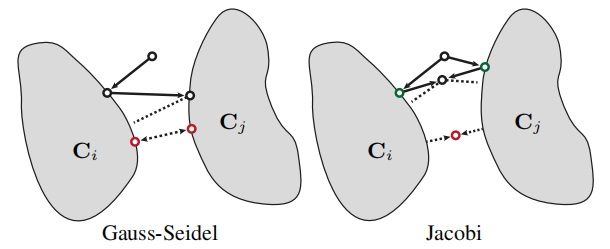
\includegraphics[width=1.0\linewidth]{./fig/Gauss-Seidel-Jacobi.jpg}
            \captionof{figure}{Gauss-Seidel-Jacobi}
        \end{center}

		PBD方法实际上是把弹簧质点系统中的弹力变为了约束,系统的刚度取决于迭代的次数,迭代次数越多时约束越强,系统的刚度也就越大,然而很难得到一个物体的力学性质和迭代次数的关系。与隐式欧拉法相比,PBD优化的目标是$E(x)$,这使得它忽略了惯性项$\frac{1}{2(\Delta t)^2}(x-\bar x)^TM(x-\bar x)$,同时它不是基于物理推导出来的,不符合物理规律。

		\section{常见的线性方程组求解方法}
		\subsection{直接法:LU 分解、LDLT 分解、Cholesky 分解}
		\begin{itemize}
			\item[$\bullet$] 代价高,得到精确解
			\item[$\bullet$] 对矩阵限制少
			\item[$\bullet$] 适合 CPU 计算
		\end{itemize}

		\subsection{迭代法:Jacobi}
		\begin{itemize}
			\item[$\bullet$] 如果需要得到精确解的话代价大,但是可以根据容差控制
			\item[$\bullet$] 要让方法收敛的话,对矩阵 有比较严格的限制(例如正定)
			\item[$\bullet$] 可使用GPU并行
			\item[$\bullet$] 实现比较容易
			\item[$\bullet$] 有很多加速算法
		\end{itemize}

        \begin{center}
            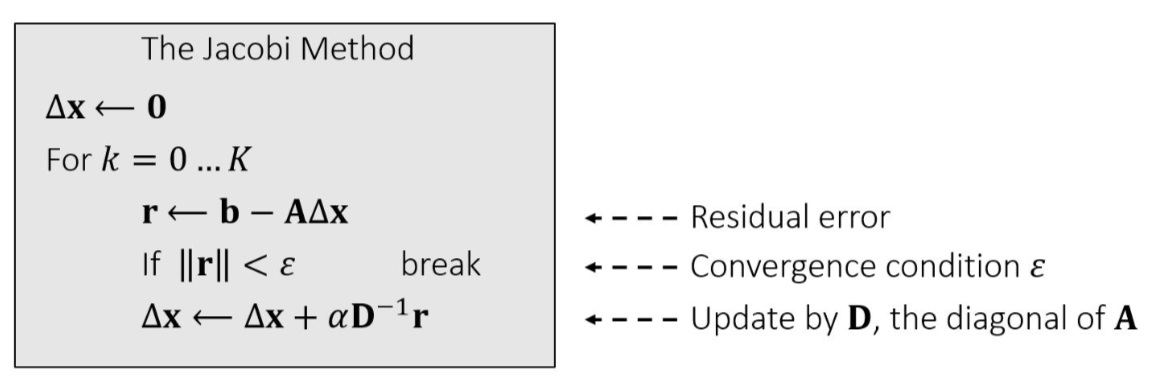
\includegraphics[width=1.0\linewidth]{./fig/Jacobi.jpg}
            \captionof{figure}{Jacobi}
        \end{center}

		\section{基于块式梯度下降的隐式欧拉法\textsuperscript{\cite{1}}}
		在隐式欧拉法中,最后需要求解一个优化问题,除了用牛顿法外,还可以用块式梯度下降的方法,与牛顿法相比它们收敛到同一结果,虽然在渐进收敛速度上比牛顿法慢,但在不追求精度的情况下,并不需要迭代到最终收敛,这个方法在单步迭代的速率上快于牛顿法,因此在初始的几步迭代中能够快速减小误差同时取得与牛顿法相似的结果。

        \begin{center}
            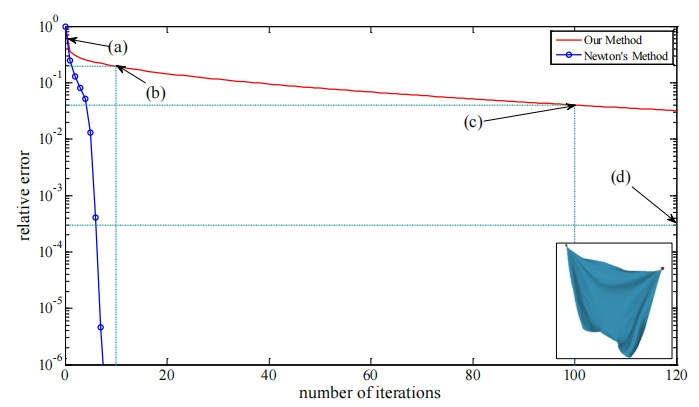
\includegraphics[width=1.0\linewidth]{./fig/块式梯度下降与牛顿法.jpg}
            \captionof{figure}{块式梯度下降与牛顿法}
        \end{center}


​		隐式欧拉法的优化目标为:
       \begin{equation}
		\Delta \pmb{p_1} =-\frac{1}{2}(\left | \pmb{p_1}-\pmb{p_2} \right |-L)\frac{\pmb{p_1}-\pmb{p_2}}{\left | \pmb{p_1}-\pmb{p_2} \right |}
		\end{equation}

		通常来说,外力的势能都不是关于位置的线性函数,但可以将其拆分为线性部分和非线性部分,将非线性部分用显式欧拉法计算,从而使整体变为线性方程,利用坐标下降的方法,交替优化非线性部分和整体。
	
		利用胡克定律(Hooke's law)的另一形式:
       \begin{equation}
			\left(\left|\left|\mathbf{p}_{1}-\mathbf{p}_{2}\right|\right|-r\right)^{2}=\operatorname*{min}_{\left|\left|\mathbf{d}\right|\right|=r}\ \left|\left|\left(\mathbf{p}_{1}-\mathbf{p}_{2}\right)-\mathbf{d}\right|\right|^{2}
		\end{equation}
	
		对于弹簧的弹性势能:
       \begin{equation}
			\frac{1}{2}\sum_{i=1}^{s}k_{i}||\mathbf{p}_{i_{1}}-\mathbf{p}_{i_{2}}-\mathbf{d}_{i}||^{2}={\frac{1}{2}}\mathbf{x}^{\mathsf{T}}\mathbf{L}\mathbf{x}-\mathbf{x}^{\mathsf{T}}\mathbf{J}\mathbf{d}
		\end{equation}

		其中:
		\begin{equation}
			{\bf L}=\left(\sum_{i=1}^{s}k_{i}{\bf A}_{i}{\bf  A}_{i}^{\mathsf{T}}\right)\otimes{\bf I}_{3},\;{\bf J}=\left(\sum_{i=1}^{s}k_{i}{\bf A}_{i}{\bf S}_{i}^{\mathsf{T}}\right)\otimes{\bf I}_{3}
		\end{equation}

		考虑到其它保守力的存在:
       \begin{equation}
			E(\mathbf{x})=\operatorname*{min}_{d\in U}~{\frac{1}{2}}\mathbf{x}^{\mathsf{T}}\mathbf{L}\mathbf{x}-\mathbf{x}^{\mathsf{T}}\mathbf{J}\mathbf{d}+\mathbf{x}^{\mathsf{T}}\mathbf{f}_{e x t}
		\end{equation}

		得到最终的优化问题:
       \begin{equation}
			\operatorname*{min}_{{{\bf x}\in{\bf R}^{3},{\bf d}\in U}}\;\;\frac{1}{2}{\bf x}^{\bf T}({\bf M}+\Delta t^2{\bf L}){\bf x}-\Delta t^2{\bf x}^{\bf T}{\bf J}{\bf d}+{\bf x}^{\bf T}{\bf b}
		\end{equation}

		从x的初始猜测(显式欧拉法的结果)开始,交替优化x和d,其中优化x时是一个凸二次最小化问题,${\bf M}+\Delta t^2{\bf L}$是一个在迭代中不变的正定矩阵,可以对其预先计算其Cholesky分解从而加快速度。

		这个方法与PBD相比,正确地考虑了惯性项$\frac{1}{2}{\bf x}^{\bf T}{\bf M}{\bf x}$的存在,同时弹簧的刚性也被包括在${\bf L}$和${\bf J}$中。

		对于阻尼的作用,可以简单将其转换为速度的百分比衰减:
       \begin{equation}
			\tilde{\mathrm{v}}_{n}\ =\ \alpha \mathrm{v}_{n}
		\end{equation}

		对于碰撞,可以直接将x移动到无碰撞的区域,这部分由碰撞响应线程实现。


		\section{投影动力学(Projective Dynamics)\textsuperscript{\cite{2}}}
		PD是一个对物理系统进行隐式欧拉积分的新方法,可以将约束转换为势能部分,将势能表示为两部分的和:

       \begin{equation}
			W({\bf q},{\bf p})=d({\bf q},{\bf p})+\delta_{\mathrm{E}}({\bf p})
		\end{equation}

		其中$\delta_{\mathrm{E}}({\bf p})$形式化了p应该位于约束流形上的要求,$d({\bf q},{\bf p})$用于衡量p和q之间的距离,对p最小化方程(30)等价于寻找q在约束流形上的投影,因此对于材料模型$\Psi$产生的弹性势$W({\bf{q}})\,\,=\,\,\Psi({\bf{E}}({\bf{q}}))=\operatorname*{min}_{\mathbf{P}}W(\mathbf{Q},\mathbf{p})$

        \begin{center}
            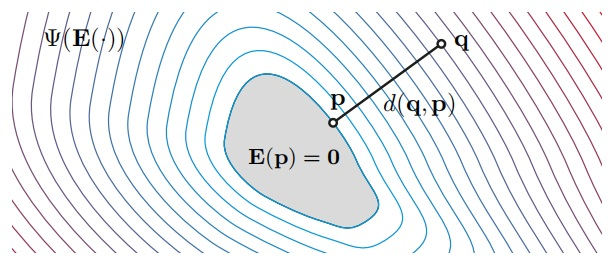
\includegraphics[width=1.0\linewidth]{./fig/材料弹性势.jpg}
            \captionof{figure}{材料弹性势}
        \end{center}

		将势能代入隐式欧拉积分中,采取交替优化的方法,先基于当前的q求出p,再根据新的p更新q,反复迭代直到收敛。

		$d({\bf q},{\bf p})$可取为简单的线性函数,这样在p固定时优化q变为线性优化问题,从而可以快速计算,而非线性的部分在优化p的过程中进行,这与[1]的思想类似。

		例如使用以下的二次距离度量:
       \begin{equation}
			W({\bf q},{\bf p})\,=\,\frac{w}{2}\|\mathrm{A}{\bf q}-{\bf B}{\bf p}\|_{F}^{2}+\delta_{\bf C}({\bf p})
		\end{equation}

		在优化p时,优化问题为:
		\begin{equation}
			\operatorname*{min}_{\mathbf{p}_{i}}{\frac{w_{i}}{2}}\|\mathbf{A}_{i}\mathbf{S}_{i}\mathbf{q}-\mathbf{B}_{i}\mathbf{p}_{i}\|_{F}^{2}+\delta_{\mathbf{C}_{i}}(\mathbf{p}_{i})
		\end{equation}
		
		在优化q时,由于为线性优化,由极值点梯度为0得到
       \begin{equation}
			(\frac{\mathrm{M}}{h^{2}}+\sum_{i}w_{i}\mathrm{S}_{i}^{T}{\bf A}_{i}^{T}{\bf A}_{i}{\bf S}_{i}){\bf q}=\frac{\mathrm{M}}{h^{2}}{\bf s}_{n}+\sum_{i}w_{i}{\bf S}_{i}^{T}{\bf A}_{i}^{T}{\bf B}_{i}{\bf p}_{i}
		\end{equation}

		此时可以选用直接法或迭代法求解该线性方程。

		\section{SOR在PBD算法上的应用\textsuperscript{\cite{3}}}

		在优化视角下,PBD算法等价于:
		\begin{equation}
		\begin{split}
			&\mathrm{minimize}\quad \frac{1}{2}\Delta x^{T}M\Delta x\\ 
			&\mathrm{subject\;to}\quad C_{i}(x+ \Delta x)=0,\quad i=1,\cdot\cdot,n			
		\end{split}
		\end{equation}

		也就是寻找满足约束条件的动能的最小变化,这与高斯最小拘束原理一致。

		由于约束通常是非线性非凸函数,使用顺序二次规划(SQP)进行,求解二次最小化序列:
		\begin{equation}
		\begin{split}
			&\mathrm{minimize}\quad\mathrm{\frac{1}{2}}\Delta{\bf x}^{T}{\bf M}{\bf x}\\
			&\mathrm{subjec \; to}\quad J\Delta x={\bf b}		
		\end{split}
		\end{equation}
		
		这种类型的问题可以转化为以下的最优化条件:
		\begin{equation}
		\begin{split}
			&M\Delta x=\mathrm{J}^{T}\lambda\\ 
			&J\Delta x={\bf b}	
		\end{split}
		\end{equation}
		其中第一个式子由拉格朗日乘数法得到,第二个式子为可行性条件。

		从中消除$\Delta x$得到:
       \begin{equation}
			\left[\mathbf{JM}^{-1}\mathbf{J}^{T}\right]\lambda=\mathbf{b}
		\end{equation}
		这是一个线性方程,可以使用迭代法求解。

		为了解决Gauss-Seidel方法不能并行的问题,可以先并行地处理每个约束,在迭代结束时将它们的均值作为最终的结果,并引入一个全局参数控制SOR的速率:
       \begin{equation}
			\Delta\tilde{\bf x}_{i}=\frac{\omega}{n_{i}}\Delta{\bf x}_{i}
		\end{equation}

		它不能保证动量守恒,但一般视觉误差并不明显。

		利用约束平均可以避免迭代法在矩阵不满足要求时不收敛的问题,通常$1 \le \omega \le 2$,不需要额外的欠松弛($\omega < 1$),因为约束平均已经足以避免发散。

		在实践中,通常希望某些类型的约束优先于其它类型的约束,可以分组处理约束,在处理下一个约束组前,将累计的位移变化立即应用到当前位移上。

		\section{PD算法的Chebyshev加速\textsuperscript{\cite{4}}}

		注意到PD算法的收敛性与线性系统高度相似,因此可以使用Chebyshev加速来加速PD算法的收敛,其中谱半径从其收敛速度中估计得到。

		Chebyshev加速方法易于实现,且与GPU加速兼容,其算法流程如下
        \begin{center}
            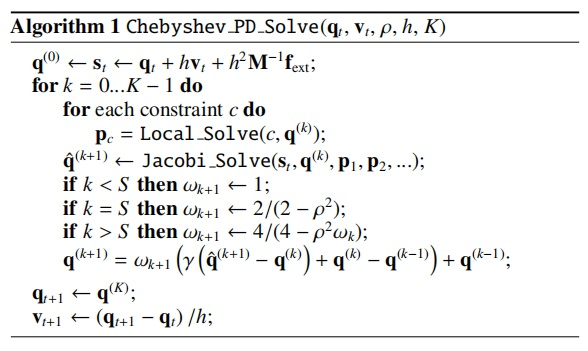
\includegraphics[width=1.0\linewidth]{./fig/chebyshev.jpg}
            \captionof{figure}{chebyshev}
        \end{center}

		Chebyshev加速方法还需要谱半径$\rho$,设估计的谱半径为$\hat \rho$,当$\hat \rho = 0$时,这个方法退化为不加速的迭代法,当$0 < \hat \rho < \rho$时,随着$\hat \rho$的增大收敛速度提升,一旦$\rho < \hat \rho$,会产生震荡,因此需要准确估计谱半径大小。

		由于PD有类似于线性系统的收敛性,把$\rho$作为每个问题中的常数,通过预模拟以估计$\rho$。首先将$\rho$初始化为$\left|\left|\mathbf{e}^{(K)}\right|\right|_{2}/\left|\left|\mathbf{e}^{(K-1)}\right|\right|_{2}$,其中误差被定义为$\mathrm{e}^{(k)}=\nabla\epsilon(\mathbf{q}^{(k)})$,然后多次调整$\rho$并进行仿真,找到收敛速度最大的$\rho$。
        \begin{center}
            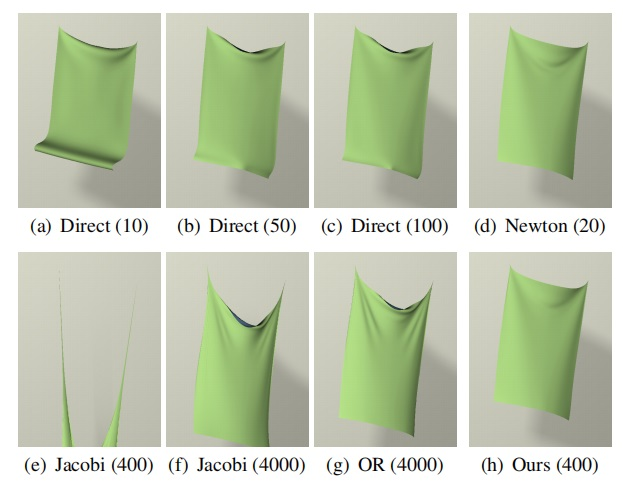
\includegraphics[width=1.0\linewidth]{./fig/Chebyshev加速对比.jpg}
            \captionof{figure}{Chebyshev加速对比}
        \end{center}

		如(c)所示直接求解器在100次迭代后仍存在卷边伪影,同时Jacobi求解器收敛缓慢,而(h)中经过Chebyshev加速的Jacobi求解器与牛顿模拟方法高度相似。

		\section{XPBD\textsuperscript{\cite{5}}}

		PBD算法中时间步长和迭代次数决定了物体的刚性,在复杂的系统中,由于参数之间的耦合,难以单独改变一个物体的刚性。在这篇文章中,提出了拓展的PBD算法(XPBD),显式引入弹性势能,从而通过弹性势能来确定物体刚性。

		弹性势能场为:
       \begin{equation}
			U({\bf x})={\frac{1}{2}}{\bf C}({\bf x})^{T}\alpha^{-1}{\bf C}({\bf x})
		\end{equation}

		由此所产生的弹性力为:
       \begin{equation}
			\mathbf{f}_{e l a s t i c}=-\nabla_{\mathbf{x}}U^{T}=-\nabla\mathbf{C}^{T}\alpha^{-1}\mathbf{C}
		\end{equation}

		引入拉格朗日乘子将其分解得到:
       \begin{equation}
			\lambda_{e l a s t i c}=-\tilde{\alpha}^{-1}{\bf C}({\bf x})
		\end{equation}
		其中$\widetilde{\alpha}=\frac{\alpha}{(\Delta t)^2}$

		得到离散的运动方程:
		\begin{equation}
		\begin{split}
			&\mathrm{M}({\bf x}^{n+1}-\tilde{\bf x})-\nabla{\bf C}({\bf x}^{n+1})^{T}\lambda^{n+1}=\mathrm{O}\\ 
			&{\mathbf C}({\mathbf x}^{n+1})+\widetilde{\alpha}\lambda^{n+1}={\mathbf0}
		\end{split}
		\end{equation}

		将两式分别记为g和h,需要找到x和$\lambda$满足:
		\begin{equation}
		\begin{split}
			&\mathbf{g}(\mathbf{x},\lambda)=\mathbf{0}\\ 
			&\mathbf{h}(\mathbf{x},\lambda)=\mathbf{0}
		\end{split}
		\end{equation}

		得到以下线性牛顿子问题:
		\begin{equation}
		\left[\begin{array}{cc}
		\mathbf{K} & -\nabla \mathbf{C}^{T}\left(\mathbf{x}_{i}\right) \\
		\nabla \mathbf{C}\left(\mathbf{x}_{i}\right) & \tilde{\boldsymbol{\alpha}}
		\end{array}\right]\left[\begin{array}{l}
		\Delta \mathbf{x} \\
		\Delta \boldsymbol{\lambda}
		\end{array}\right]=-\left[\begin{array}{l}
		\mathbf{g}\left(\mathbf{x}_{i}, \boldsymbol{\lambda}_{i}\right) \\
		\mathbf{h}\left(\mathbf{x}_{i}, \boldsymbol{\lambda}_{i}\right)
		\end{array}\right]
		\end{equation}

		现在使用两个近似方法以简化计算的实现,假设$\mathbf{K} \approx \mathbf{M}$,并且$\mathbf{g}\left(\mathbf{x}_{i}, \boldsymbol{\lambda}_{i}\right) \approx 0$:
		\begin{equation}
		\left[\begin{array}{cc}
		\mathbf{M} & -\nabla \mathbf{C}^{T}\left(\mathbf{x}_{i}\right) \\
		\nabla \mathbf{C}\left(\mathbf{x}_{i}\right) & \tilde{\boldsymbol{\alpha}}
		\end{array}\right]\left[\begin{array}{l}
		\Delta \mathbf{x} \\
		\Delta \boldsymbol{\lambda}
		\end{array}\right]=-\left[\begin{array}{l}
		0 \\
		\mathbf{h}\left(\mathbf{x}_{i}, \boldsymbol{\lambda}_{i}\right)
		\end{array}\right]
		\end{equation}


		最终得到新的迭代方程:
       \begin{equation}
		\begin{split}
			\Delta{\bf x}={\bf M}^{-1}\nabla\mathrm{C}({\bf x}_{i})^{T}\Delta\lambda \\
			\Delta\lambda_{j}=\frac{-C_{j}({\bf x}_{i})-\bar{\alpha}_{j}\lambda_{i j}}{\nabla C_{j}\mathrm{M}^{-1}\nabla(C_{j}^{T}+\tilde{\alpha}_{j}}
		\end{split}
		\end{equation}

		XPBD的算法流程如下
        \begin{center}
            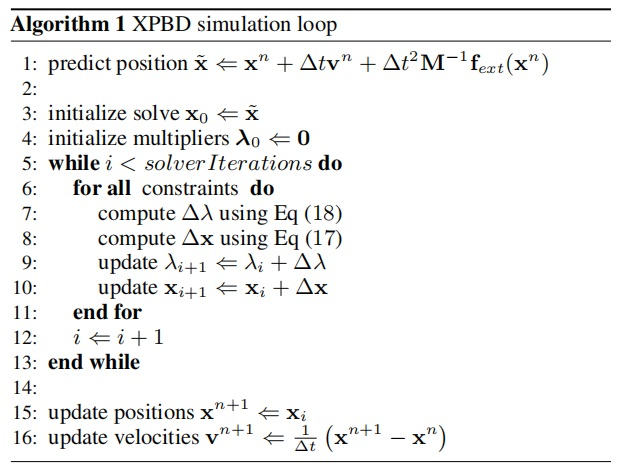
\includegraphics[width=1.0\linewidth]{./fig/XPBD算法.jpg}
            \captionof{figure}{XPBD算法}
        \end{center}

		\section{多重网络\textsuperscript{\cite{6}}}
		多重网格法是迭代方法的一种,可用于求解线性方程组。

		一般的迭代法在求解线性方程组$A\phi=b$基于固定的步长进行迭代得到$\phi ^n$,对残差$r=b-A\phi^{n}$进行傅里叶变换可以把它们分解成一系列不同频率的残差,在迭代中对于频率较高的残差消除的较快,对频率低的残差消除的慢。可以通过增大步长来等价地提高频率,从而消除低频误差,但步长大时精度较低,因此可以在不同的步长上交替进行,在保持精度的同时加快误差消除,这被称为多重网格法。

		先在细网格上迭代使得频率大的误差衰减,剩下误差中频率较小的部分;再将误差中频率较小的部分作为方程组的右侧,在粗网格上迭代,使得频率较小的误差也能快速地衰减;最后为了保证精度,将粗网格上迭代的结果和细网格上的结果加总之后,作为初始猜测值再在细网格上迭代。如此循环往复。因为先由细到粗,后由粗到细,网格转换的路径形似 V 字,所以该方法被称为 V-Cycle Multigrid。除此之外还有 F-cycle multigrid 和 W-cycle multigrid。他们的基本思想相同。
        \begin{center}
            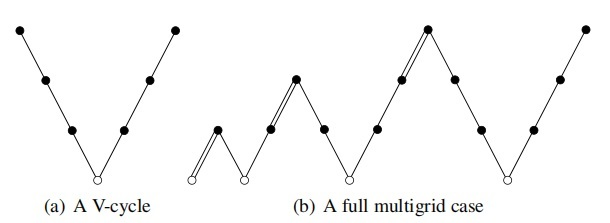
\includegraphics[width=1.0\linewidth]{./fig/multigrid.jpg}
            \captionof{figure}{multigrid}
        \end{center}
		
		图中黑色圆点代表平滑,白色圆点代表精确求解器,\textbackslash 和/代表限制和插值,//代表高阶插值,限制和插值用于粗细网格结果之间的映射。

		非线性FMG(full multigrid)的工作结构如下:
        \begin{center}
            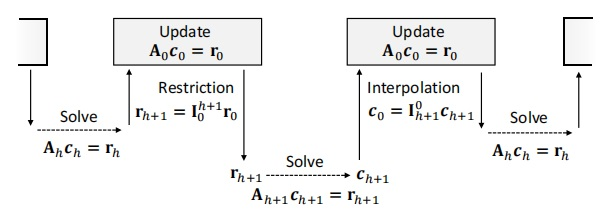
\includegraphics[width=1.0\linewidth]{./fig/非线性FMG.jpg}
            \captionof{figure}{非线性FMG}
        \end{center}

		利用多重网格,可以加速布料仿真中迭代法求解线性方程收敛的速度。


		\section{基于深度学习的服装CG生成\textsuperscript{\cite{7}}}
		衣物的生成通常通过物理模拟来实现,通过设置不同的物理参数,可以生成不同材质、形状的衣服。但是,为一个CG来生成衣服需要对于每一帧动作指定对应的物理参数,而这个参数和动作,前后帧都是有关系的。

		为了减少参数设置的工作量,需要在关键帧之间自动生成对应的衣服,但关键帧之间的运动可能非常复杂,衣服的生成无法直接通过插值得到,因此通过深度学习的方式找到衣服所对应的潜在空间,从而将衣物应用到不同的动作上。
        \begin{center}
            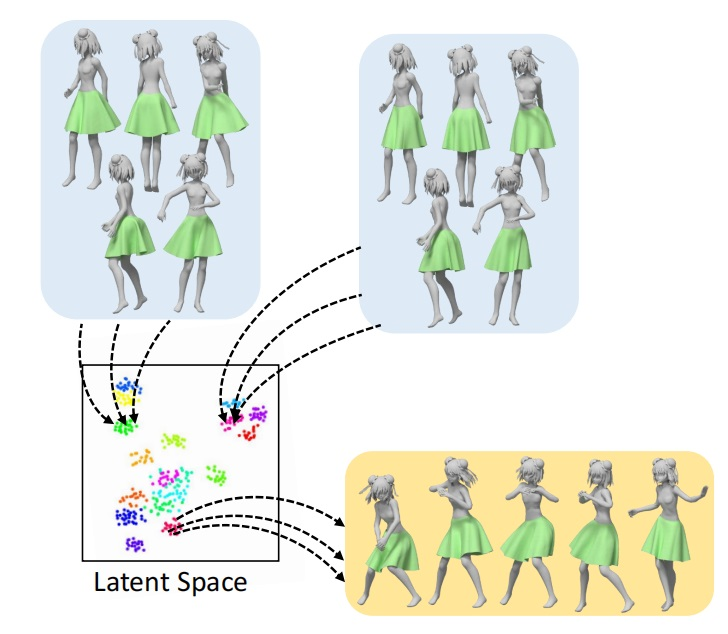
\includegraphics[width=1.0\linewidth]{./fig/潜在空间.jpg}
            \captionof{figure}{潜在空间}
        \end{center}

		一个潜在空间上的点可以在不同的动作下对应于不同的衣物。

		首先使用多层感知机(MLP)对服装网格进行编码与解码,将其进行降维
        \begin{center}
            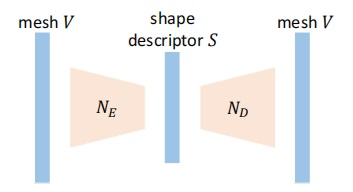
\includegraphics[width=1.0\linewidth]{./fig/多层感知机.jpg}
            \captionof{figure}{多层感知机}
        \end{center}

		它的损失函数为:
       \begin{equation}
			||V-N_{D}(N_{E}(V))||_{2}+\omega\cdot||\Delta(V)-\Delta(N_{D}(N_{E}(V)))|_{2}
		\end{equation}

        \begin{center}
            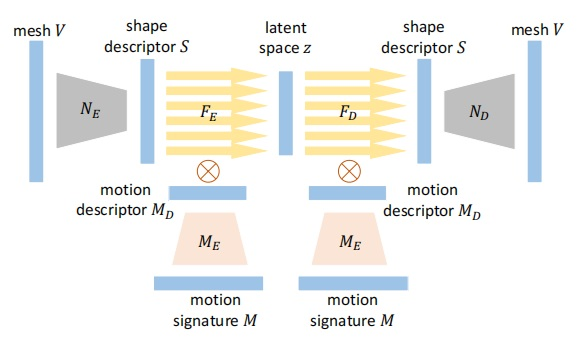
\includegraphics[width=1.0\linewidth]{./fig/auto-encode.jpg}
            \captionof{figure}{auto-encode}
        \end{center}

​		通过自动编码器进行服装网格与形状描述符之间的编码与解码,运动标签与运动描述符之间的编码与解码,将服装描述符和运动描述符降维到潜在空间中,其中运动描述符作为形状描述符到潜在空间的编码器的子网权重,再通过新的运动描述符重新变换回服装网络。

        \begin{center}
            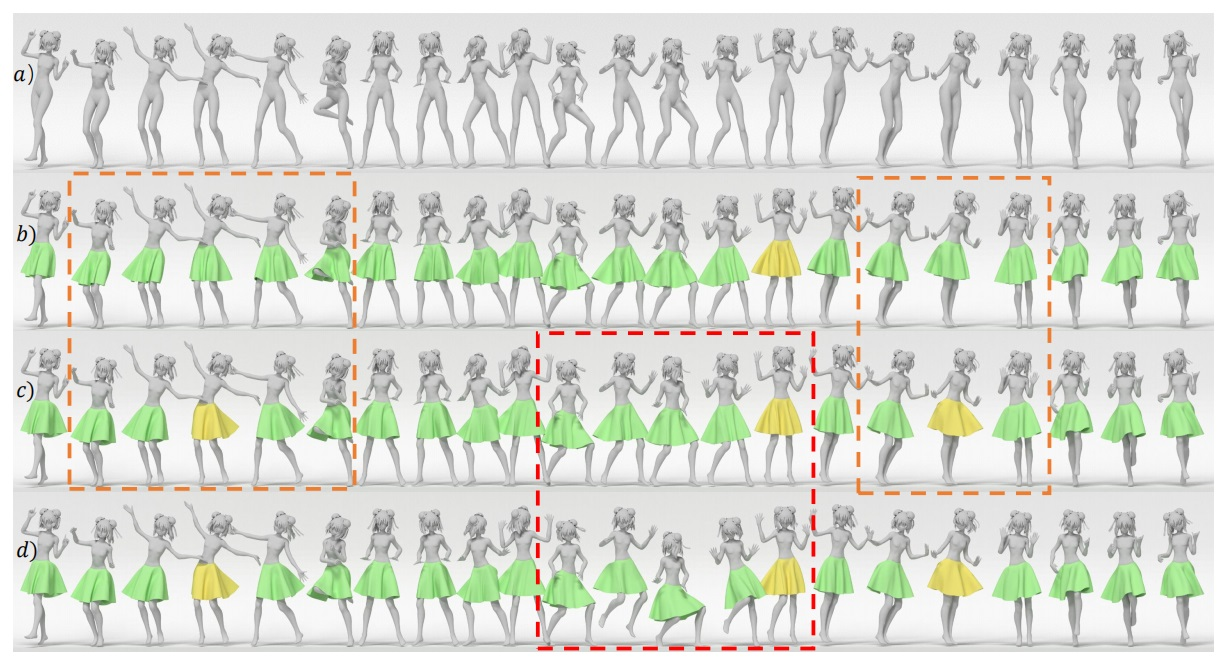
\includegraphics[width=1.0\linewidth]{./fig/animation.jpg}
            \captionof{figure}{animation}
        \end{center}

		这是一个半自动的服装动画创作工作流程。给定一个身体动画序列(a),艺术家选择一个关键帧(用黄色标记),并输入该帧(b)的服装形状,系统学习该设计的内在属性,并自动将该设计传播到其他帧(用绿色标记)。艺术家可以通过插入新的关键帧(用黄色标记)和编辑关键帧的服装形状来进一步调整服装动画(c)。然后,通过链接关键帧与合理的过渡(用橙色框突出显示),可以自动更新动画序列。工作流程还允许艺术家在构图过程中修改身体动画(用红色框标记),因为我们的系统可以从底层的身体运动推断出服装的形状(d).

		\section{Incremental Potential Contact\textsuperscript{\cite{8}}}
		为了处理仿真中产生的碰撞,可以将碰撞视为一种约束,从而转化为优化问题。一般的隐式欧拉优化目标为:
       \begin{equation}
		\begin{split}
			&E(x,x^{t},v^{t})=\frac{1}{2}(x-\hat{x})^{T}{\cal M}(x-\hat{x})-h^{2}x^{T}f_{d}+h^{2}\Psi(x)\\
			&\hat{x}=x^{t}+h v^{t}+h^{2}M^{-1}f_{e}\\
			&x^{t+1}=\arg\operatorname*{min}_{x}E(x,x^{t},v^{t}),\quad x^{\tau}\in\cal{A}
		\end{split}
		\end{equation}
		其中$\cal{A}$为不发生碰撞的空间区域

		IPC方法将约束条件融合到目标函数中:
       \begin{equation}
			\arg\operatorname*{min}_{x}E(x)=\frac12\|x-x^{*}\|_{M}^{2}+h^{2}\Psi(x)+\kappa\sum_{k\in C}b(d_{k}(x))
		\end{equation}

		其中b是一个障碍函数,当$0 < d < \hat d$时靠的越近会受到越大的阻力
       \begin{equation}
			b(d_{k}(x)=\left\{\begin{array}{l l}{{-\,(d-\hat{d}\,)^{2}\ln(\frac{d}{\hat{d}}),\quad}}&{{0< d< \hat{d}}}\\ {{0,\quad}}&{{d\geq\hat{d}}}\end{array}\right.
		\end{equation}

        \begin{center}
            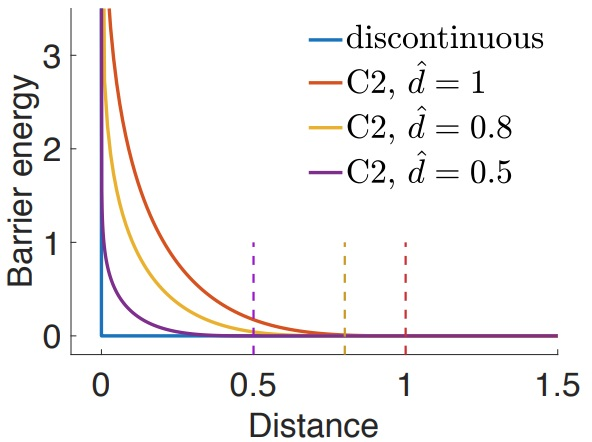
\includegraphics[width=1.0\linewidth]{./fig/障碍势能.jpg}
            \captionof{figure}{障碍势能}
        \end{center}

		\section{高分辨率布料褶皱模拟\textsuperscript{\cite{9}}}
		传统的布料仿真使用非结构化的三角形网络,但这会带来巨大的内存开销和计算成本,在较高分辨率下三角形网络的灵活性不再重要,可以使用规则网络,提高内存访问的效率。

		在高分辨率下模拟布料褶皱的流程如下
        \begin{center}
            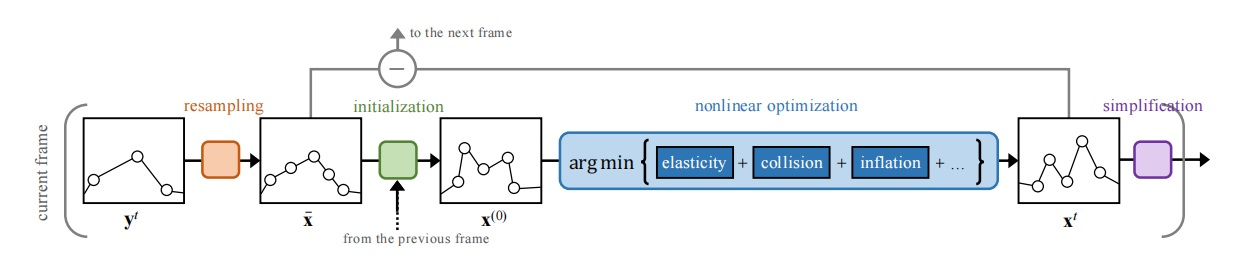
\includegraphics[width=1.0\linewidth]{./fig/褶皱模拟流程.jpg}
            \captionof{figure}{褶皱模拟流程}
        \end{center}
		输入一个非结构化的网络,通过一个规则网络重新采样,然后运行一个初始化步骤来估计网格上的褶皱,通过非线性优化来生成褶皱的细节,最终将褶皱简化以便下一步处理。

		为了提升收敛速度,使用GPU来并行处理,可以在不重叠的GPU线程块中使用共享内存,这是由网格分区所自然创建的。但在每次迭代中每个块都需要将其部分从全局内存加载到共享内存中,如果块能够覆盖全部顶点,那就可以一次性加载共享内存,在顶点较多时,如果我们只为同一个不重叠的GPU块中的线程运行内部迭代,就可以重用只加载一次的共享内存数据。

		利用GPU加速的块式梯度下降算法如下
        \begin{center}
            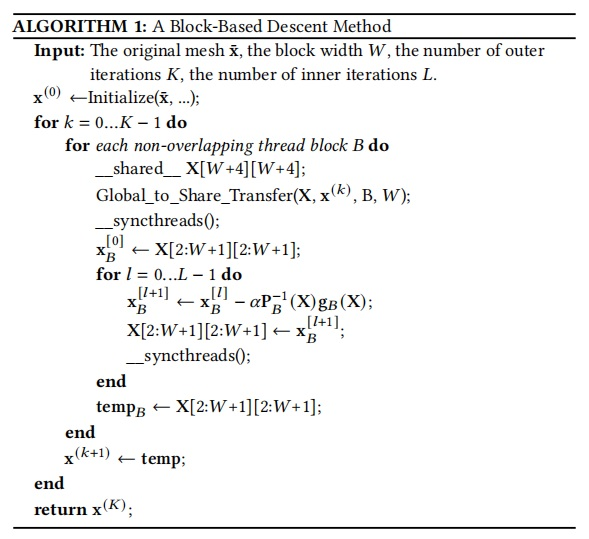
\includegraphics[width=1.0\linewidth]{./fig/gpu.jpg}
            \captionof{figure}{gpu}
        \end{center}

		\section{总结}
		布料是一种在形变时会产生弹性势能的物体,在布料仿真时需要计算形变时弹性势能对状态的影响,通常仅考虑相邻顶点之间的弹性势能。布料仿真的模型较为单一,因此近十年的研究方向主要在于如何设计新的算法或是采用一些优化策略提升仿真速度与效果,在此基础上提出了PD、XPBD、IPC等方法构造不同的优化目标以取得更好的效果,以及应用数值计算方法(如块式梯度下降、SOR、Chebyshev加速)以加速原有的算法,还有基于深度学习半自动生成服装CG的新的研究方向。

		\begin{thebibliography}{8}
			\bibitem{1}Liu T ,  Bargteil A W ,  O'Brien J F , et al. Fast Simulation of Mass-Spring Systems[J]. ACM Transactions on Graphics, 2013, 32(6):209:1-7.
			\bibitem{2}Sofien, Bouaziz, Sebastian, et al. Projective dynamics: fusing constraint projections for fast simulation[J]. ACM Transactions on Graphics (TOG) - Proceedings of ACM SIGGRAPH 2014, 2014, 33(4).
			\bibitem{3}Macklin M ,  Mueller M ,  Chentanez N , et al. Unified particle physics for real-time applications[J]. Acm Transactions on Graphics, 2014, 33(4CD):1-12.
			\bibitem{4}Wang H . A Chebyshev Semi-Iterative Approach for Accelerating Projective and Position-based Dynamics[J]. ACM Transactions on Graphics, 2015, 34(6cd):246.1-246.9.
			\bibitem{5}Macklin M , M Müller,  Chentanez N . XPBD: Position-Based Simulation of Compliant Constrained Dynamics[C]// Motion In Games 2016. ACM, 2016.
			\bibitem{6}Wang Z ,  Wu L ,  Fratarcangeli M , et al. Parallel Multigrid for Nonlinear Cloth Simulation[J]. Computer Graphics Forum, 2018, 37(7):131-141.
			\bibitem{7}Wang T Y ,  Shao T ,  Fu K , et al. Learning an intrinsic garment space for interactive authoring of garment animation[J]. ACM Transactions on Graphics, 2019, 38(6):1-12.
			\bibitem{8}Li M ,  Ferguson Z ,  Schneider T , et al. Incremental Potential Contact: Intersection-and Inversion-free, Large-Deformation Dynamics[J]. ACM Transactions on Graphics, 2020, 39(4):20.
			\bibitem{9}Wang H . GPU-based simulation of cloth wrinkles at submillimeter levels[J]. ACM Transactions on Graphics, 2021, 40(4):1-14.
		\end{thebibliography}
    \end{multicols}%结束分栏

\Title{Cloth Simulation: A Decade of Acceleration}
\Author{Chen Wang}
\Institute{(University of Science and Technology of China, School of Computer Science and Technology, PB20111696)}
\Maketitle
\begin{enabstract}
	This article mainly introduces the common methods of cloth simulation and the cutting-edge research of cloth simulation in the past ten years, including performance optimization of existing algorithms, new simulation algorithms, and parallel implementation of algorithms on GPU, and summarizes the current frontier direction of cloth simulation.

\end{enabstract}
\enkeywords{Cloth Simulation}


\end{document}